\documentclass{article}

% Language setting
% Replace `english' with e.g. `spanish' to change the document language
\usepackage[english]{babel}

% Set page size and margins
% Replace `letterpaper' with `a4paper' for UK/EU standard size
% \usepackage[letterpaper,top=2cm,bottom=2cm,left=3cm,right=3cm,marginparwidth=1.75cm]{geometry}
\usepackage[letterpaper,top=2cm,bottom=2cm,left=3cm,right=3cm]{geometry}

% Useful packages
\usepackage{amsmath,amssymb}
\usepackage{graphicx}
\usepackage[colorlinks=true, allcolors=blue]{hyperref}
\usepackage{cite}



%\setlength{\parindent}{0pt}

\title{%

\includegraphics[width=0.2\textwidth]{dauphine.png}~ 
\\[0.3cm]
Optimization Project - IASD 2022-23 \\ }
\author{Maximilien Wemaere}
\date{}

\begin{document}

\maketitle

\section*{Introduction}

This project aims to implement the different algorithms seen in the optimization syllabus of the M2-IASD program. All the codes are available at: % github link

\section{Gradient Descent}

\subsection{Dataset presentation}
    The data used is from the dataset \textit{Life Expectancy} which contain different factors influencing life expectancy and is provided by the World Health Organization. The aim is to predict the life expectancy (LE) of a country with the different factors of it.
    
    There is 22 column, and we delete 3 of them because they will not help to determine the LE('country','year,''status') plus the LE column. So there is 18 dimensions to our optimization problem. 

    We have 2938 points in our dataset, but if we drop all rows with a a NA value, we have only 1649 points. So we use a training set of 1349 points and a test set of 300 points.

    The model chosen is a linear regression, so we have an optimization problem with 18 parameters.

    Before we start, we normalize our data by setting the mean to 0 and the standard deviation to 1.

    Then we print our correlation matrix: 

    \begin{figure}[!h]
    \centering
    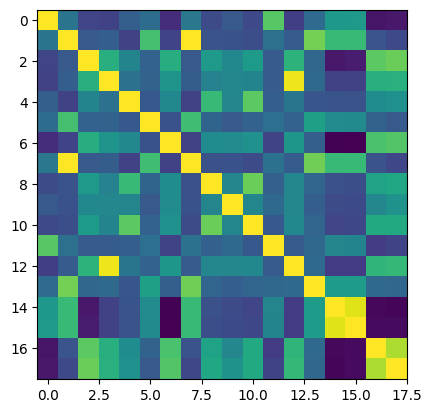
\includegraphics[width=0.4\textwidth]{images/corr.png}
    \caption{Correlation Matrix}
    \label{fig:res}
    \end{figure}

    We can see some high correlation between columns, such as Infant deaths and under-five death or percentage expenditure and GDP (which is pretty logic).

\subsection{Gradient descent}
    We implement gradient descent, and we test it with a learning rate of $1/||A||_{2}^2$ which is theoretically optimal, the value here is: $1.27e-4$. We add a small ridge penalty with a coefficient of $2.3e-3$. The algorithm stop when the gradient is close enough to 0. Here it stop with a loss of $6.9$ after 9 iterations (epochs).

    \begin{figure}[!h]
    \centering
    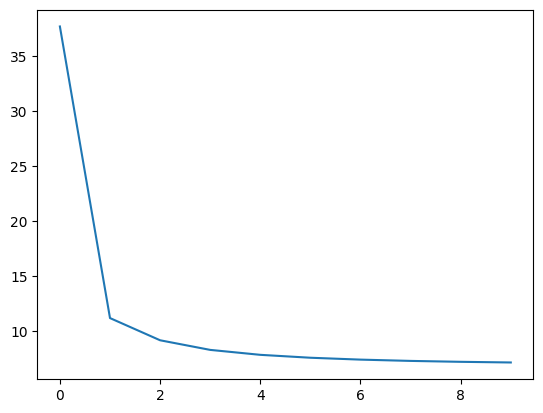
\includegraphics[width=0.4\textwidth]{images/loss1.png}
    \caption{loss evolution with GD}
    \label{fig:loss1}
    \end{figure}

    Then we vary the learning rate (or step-size) around the theoretical optimal step and we print the evolution of the loss:

     \begin{figure}[!h]
    \centering
    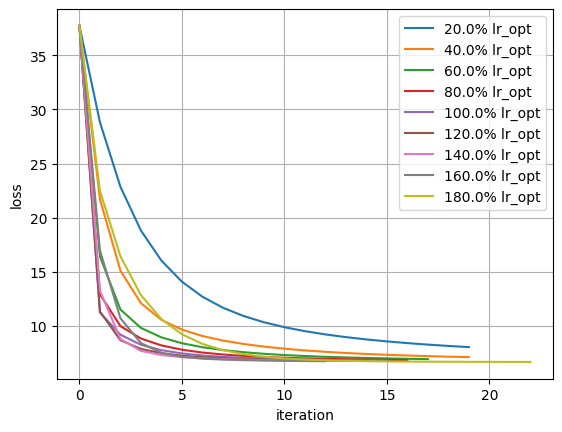
\includegraphics[width=0.4\textwidth]{images/loss2.png}
    \caption{loss evolution with different step-sizes}
    \label{fig:loss2}
    \end{figure}   

    As we expected the best learning rate is more or less the theoretical one which stop here the first, after a dozen of iterations.

    Finally we vary the coefficient of the ridge penalty. 
    
     \begin{figure}[!h]
    \centering
    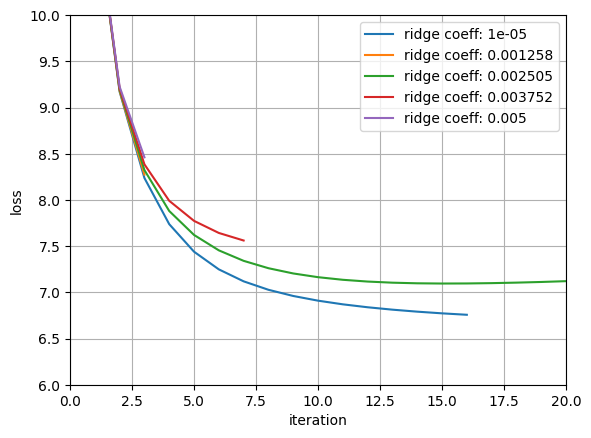
\includegraphics[width=0.4\textwidth]{images/loss3.png}
    \caption{loss evolution with different ridge penalties}
    \label{fig:loss3}
    \end{figure}   

    Here the best ridge coefficient is 0.05, if we use a higher coefficient, the algorithm do not converge and if we use a smaller the algorithm converge more slowly. So fro each optimization problem we have to find this equilibrium: the largest coefficient of ridge penalty such as the algorithm converges


    
\section{Automatic differentiation}

\section{Stochastic Gradient}
    \subsection{SG without batch}

    First we implement the Stochastic gradient algorithm without batches. In the same setting (problem, learning rate, hyperparameters) than the gradient descent, our algorithm stop after 2600 iterations (which is equivalent to 2600/1349 = 2 epoch so 2 iteration of a GD). So SG algorithm is faster than the GD one but the finakl loss is $9.6$ so worse than the GD which was $6.9$.
    
    But if we change the hyperparameter $\epsilon$ which is the minimal gradient to stop the algorithm, and we diminish it we have better results: final loss of $7.2$ after 10 epochs. This confirm the theory: SG tend to converge faster than GD but is less precise.
    \begin{figure}[!h]
    \centering
    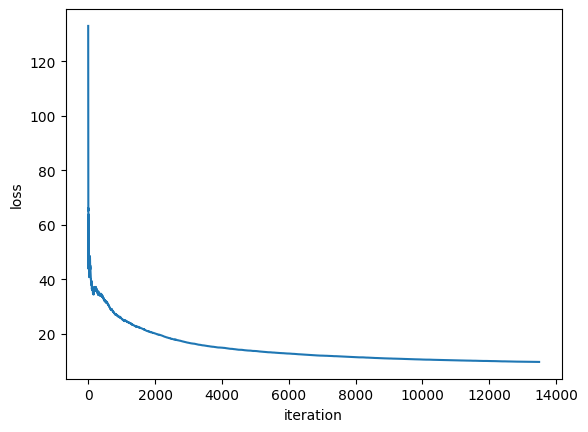
\includegraphics[width=0.4\textwidth]{images/sg1.png}
    \caption{loss evolution with SG}
    \label{fig:sg1}
    \end{figure}      



    \subsection{Batch SG}

    Now we implement a batch size, and for different batch size we print an empirical mean of the final loss (with 30 samples) and we print it:

    \begin{figure}[!h]
    \centering
    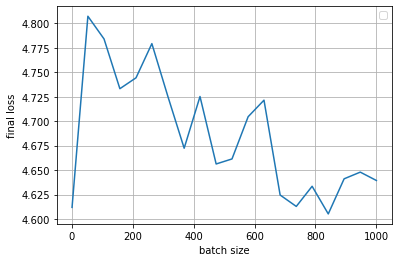
\includegraphics[width=0.4\textwidth]{images/sg2.png}
    \caption{loss evolution with different batch sizes}
    \label{fig:sg1}
    \end{figure}      

    \subsection{Stochastic Variance-Reduced Gradient}

    We have then implemented the SVRG method to compare it with the standard SG method.
 %%%% to dooo

    


\section{Convexity and constrained optimization}

\section{Proximal gradient and LASSO}

\section{Large-scale and distributed optimization}

\section{Advanced topics on gradient descent}




\clearpage
\bibliographystyle{apalike}
\bibliography{refs}


\end{document}